\documentclass{book}
\usepackage[utf8]{inputenc}
\usepackage{indentfirst}	% make indent in first paragraph
\usepackage{bm}
\usepackage{geometry}		% to make typesettings like margins
\usepackage{mathrsfs}
\usepackage{amssymb}
\usepackage{hyperref}

\usepackage{natbib}			% to insert citations
\usepackage{xcolor}			% extend the colors can be used
\usepackage{calrsfs}		% caligraphy font family

\usepackage{bibentry}		% package used to insert full citation in body text
\makeatletter 
\renewcommand\BR@b@bibitem[2][]{\BR@bibitem[#1]{#2}\BR@c@bibitem{#2}}
\makeatother
\nobibliography*

\usepackage{setspace}		% set space for comment bullet

\usepackage{graphicx}		% to insert image
\graphicspath{ {images/} }

\usepackage[framemethod=default]{mdframed}
\usepackage{showexpl}
\mdfdefinestyle{comment}{
linecolor=gray,leftmargin=60,
rightmargin=40,
backgroundcolor=gray!10,
innertopmargin=4pt,
topline=false,leftline=false,bottomline=false,rightline=false}

\usepackage[english]{babel}
\renewcommand{\baselinestretch}{1.5}

\usepackage{tocbibind}		% to add toc and bib into table of content
\usepackage{bookmark}	% to separate the last chapter from previous ones

\usepackage{amsthm}
\makeatletter
\def\th@plain{%
  \thm@notefont{}% same as heading font
  \itshape % body font
}
\def\th@definition{%
  \thm@notefont{}% same as heading font
  \normalfont % body font
}


\theoremstyle{plain}
\newtheorem{thm}{Theorem}[section] % reset theorem numbering for each chapter
\theoremstyle{definition}
\newtheorem{defn}{Definition}[section] % definition numbers are dependent on theorem numbers
\newtheorem{exmp}{Example}[section] % same for example numbers
\newtheorem{lemma}[thm]{Lemma}
\newtheorem{prop}[thm]{Proposition}
\newtheorem{obs}{Observation}

\newenvironment{myproof}
{\noindent\textit{Proof:}}{\hfill$\square$}

\citestyle{chicago}
\geometry{letterpaper, margin=1in}
% \setlength\parindent{0pt} % to cancel indent


% A list of new commands
\newcommand{\R}{\mathbb{R}}			% depends on the package amssymb
\newcommand{\F}{\mathcal{F}}
\newcommand{\myline}{\vspace{3mm} \hrule \vspace{4mm}}



\usepackage{amsmath}
\DeclareMathOperator*{\argmin}{arg\,min}




\title{Paper Notes}
\author{Kaida Zhang}
\date{}

\begin{document}

% \maketitle

\tableofcontents{}
\label{toc}
\setcounter{tocdepth}{1}			% show only parts, chapters, and sections in content


\part{Economics}
\label{part:economics}

\chapter{Econometrics}
\label{cha:econometrics}


\section{Low and Meghir, 2017, JEP} % (fold)
\label{sec:low_and_meghir_jep_2017}

\textbf{\bibentry{Low:2017jb}}\\

\textbf{Defining a structural model:}

A \textbf{fully specified model} make explicit assumptions about the economic actors' objectives and their economic enviroment and information set, as well as specifying which choices are being made within the model. They allow a complete solution to the individual's optimization problem as a function of current information set.
Fully specified models are particularly useful in understanding mechanism of a policy, especially when we want to estimate some long-term effects of the policy.

A \textbf{partially specified model} relies on a sufficient statistic that summarizes choices not being modeled specifically. For example, assuming that the choices is only intratemporal instead of intertemporal.

\textbf{Treatment effect models} focus on identifying a specific causal effect of a policy while saying least about the theoretical environment. The pro is the cleaness of causality. The con is the limitation in exploiting the results outside. The identification of treatment model depends on assumptions that the experienment has not been compromised and there is no spillovers from the treatment units.

A combination of fully speficied model and randomized experiments can enhance anaysis for both. Experimental evidence can be used either to validate a structural model, or to aid in the estimation process (in identification).

\textbf{Solving structural models}

This has been described in Adda and Cooper(2003) well. 
The general process is: 
1) write down the bellmand function;
2) discrete the state space and decision space;
3) use value function iteration to solve the bellman function.


% section low_and_meghir_jep_2017 (end)


\section{Lewbel, 2016, JEL} % (fold)
\label{sec:lewbel_2016_jel}

\textbf{\bibentry{Lewbel:2016wn}}\\

\url{https://www2.bc.edu/arthur-lewbel/ident-zoo-SL-Part1.pdf} 

\url{https://www2.bc.edu/arthur-lewbel/ident-zoo-SL-Part2.pdf}

are links for a ppt on this paper by Lewbel.\\

There are two kinds of identification problems. 
1. One is to identify the treatment effect, a typical example is the selection bias. The problem in these cases are that selection (determing who is treated or observed) and outcomes may be correlated. 
2. Another is to identify the true coefficient in a linear regression when regressors are measureed with error.

\subsection{Point Identification} % (fold)
\label{sub:point_identification}

We start by assuming some information $\phi$ is knowable. A simple definition of point identification is that a parameter $\theta$ is point identified if, given the model, is uniquely determined from $\phi$. Notice that this definition of point identification is recursive in some sense. To identify $\theta$, we first need to assume some $\phi$ is knowable, which means $\phi$ itself is identified. This identification of $\phi$ can only be justified by further assumptions of DGP (Data Generating Process).

For example, for a model $Y = X\theta +e$, we assume that $E(E^2)\ne0$ and $E(eX)=0$, and suppose $\phi$ includes the second order of $(Y,X)$. Then we can conclude that $\phi$ is point identified, given by $E(XY)/E(X^2)$. Notice that the identification comes from the \textit{assumptions} of model.

One common DGP is IID. Under this DGP, we can consistently indentify the distribution of observation W. Another DGP is where each data point consists of a value of X chosen from its support, then we randomly draw Y conditional on X, which is independent from other draws conditional on this X. Under this DGP, we can consistently identify $F(Y|X)$. We can also use more complicated DGPs, for example, we generally assume only the second order moments are knowable in time series. One reason is this being sufficient for identification, another reason is higher order moments become unstable over time. Assumptions over GDP are always needed, even in experienment data, and which specific assumptions to take depend on the model.


% subsection point_identification (end)

% section lewbel_2016_jel (end)


\section{Gentzkow-Kelley-Taddy, 17 WP} % (fold)
\label{sec:gentzkow_kelley_taddy_17_wp}

\noindent
\textbf{\bibentry{Gentzkow_el.al:17WP}}

An survey paper on how text analysis can be used in economic research. 
The main difficulty is the high-dimensionality of text.

\noindent
Steps to reduce dimension:
\begin{enumerate}
	\item Represent raw text $\mathcal{D}$ as a numerical array $C$
	\begin{enumerate}
		\item Divide $\mathcal D$ into individual documents $\mathcal D_i$, the level is determined by the level of $V$. For example, daily attributes or monthly attributes.
		\item Feature Selection. Drop out punctuations, numbers, HTML tags, proper names and so on. Both very common and very rare words will be excluded. And words with the same stems will be reduced to one.
		\item Limit dependence between words using N-gram. The idea is to only consider consider phrase of length n.
	\end{enumerate}
	\item Map $C$ to predicted values $\hat V$ of unknown outcomes $V$
	\item Use $\hat V$ in subsequent descriptive or causla analysis
\end{enumerate}


\textcolor{blue}{Reading not finished.
\cite{grimmer_stewart_2013} also talks this problem. worth reading}
% section gentzkow_kelley_taddy_17_wp (end)




\section{Seminar Notes} % (fold)
\label{sec:seminar_notes}

\noindent
\textbf{AI and Economics}
(\url{http://taddylab.com/slides/EconAI.pdf})

This slides procides some clear intro on why and how AI (also deep learning) can be applied in economics.
Many references provided in slides as well.

\textcolor{blue}{Not understand much. Needs further reading.}

% section seminar_notes (end)




% chapter econometrics (end)



%%%%%%%%%%%%%%%%%%%%%%%%%%%%%%%%% IO %%%%%%%%%%%%%%%%%%%%%%

\chapter{IO} % (fold)
\label{cha:io}

\section{Data and Techniques} % (fold)
\label{sec:data_and_techniques}

\subsection{Data Source} % (fold)
\label{sub:data_source}

\noindent
\textbf{Uber and Taxi}
\begin{itemize}
	\item New York Taxi and Limousine Commission Trip Data
	\begin{itemize}
		\item \url{http://www.nyc.gov/html/tlc/html/about/trip_record_data.shtml}
		\item Literature: Bian Bo (JMP)
	\end{itemize}
\end{itemize}


% subsection data_source (end)





\subsection{Techniques} % (fold)
\label{sub:techniques}

% subsection techniques (end)

\noindent
\textbf{High Resolution Satelite Data:}
\begin{itemize}
	\item Pixel is as accurate as 0.5m, much finer than the Night Light data;
	\item Use machine learning to identify the roads, cars, buildings etc;
	\item Jonathan Hersh has a paper over this. \textbf{\href{https://www.dropbox.com/s/zeph7rrch2rwfwp/PovSpace_JMP_Oct31.pdf?dl=0}{Poverty from Space: Using High Resolution Satellite Imagery for Estimating Economic Well-being and Geographic Targeting}}
\end{itemize}


\myline

\noindent
\textbf{Paralelle Computation:}
\begin{itemize}
	\item A detailed cook manual on Paralelle computation of RBC model: 

	\url{https://www.kellogg.northwestern.edu/researchcomputing/docs/ParallelComputing/ParallelizationForRBCModel.pdf}

	\item Another source: \url{https://bfi.uchicago.edu/sites/default/files/file_uploads/Lecture_Parallel_Programming_Chicago%20%282%29.pdf}
\end{itemize}

\myline

\noindent
\textbf{Text as Data:}
\begin{itemize}
	\item \href{run:resources/text_as_data}{Course Materials by Justin Grimmer}
	\item \bibentry{grimmer_stewart_2013}
	\item \bibentry{Gentzkow_el.al:17WP}
\end{itemize}



% section data_and_techniques (end)


\section{Rey and Stiglitz, 1995, RAND} % (fold)
\label{sec:rey_and_stiglitz_1995_rand}

\textbf{\bibentry{Rey:1995ft}}

For detailed proof of this paper, see Evernote.\\

\textbf{Main result:}
vertical restrains can be used to reduce interband competition. Because exclusive territories alter the perceived demand curve, making each producer believe he faces a less elastic demand curve, inducing an increase in eqm price and producer's profits even in the abscence of franchise fee. This result is different from traditional Chicago school results, which insist that exclusive terittories will increase efficiency. This difference comes from market structure. Chicago schools investigate in full competition and full monopoly producer cases, while this paper looks at duopoly producer. In full competition and full monopoly case, the competition level has already been \textit{preassumed}, while exclusive territories can reduce the competition level among producers in other cases.\\

The key for the result is the the following compound demand elastic:
\[\tilde\varepsilon(p^e):=m_1(p,p)\varepsilon_1(q,q)+m_2(p,p)\varepsilon_2(q,q) \]
where $q=q_1^r(p,p)$ (the response retail price),
$m_1(p,p)=\partial \log q_1^r(p_1,p_2)/\partial \log p_1$ (the own elasticity of retail price to producer price),
and  $m_2(p,p)=\partial \log q_1^r(p_1,p_2)/\partial \log p_2$ (the cross elasticity of retail price to producer price),
and $\varepsilon_1(q_1,q_2)=-\partial \log D^1(q_1,q_2)/q_1$ (the own elasticity of demand to retail price, positive),
and $\varepsilon_2(q_1,q_2)=-\partial \log D^1(q_1,q_2)/q_2$ (the cross elasticity of demand to retail price, negative).

In the above equation, it is very reasonable to think $0<m_1<1$ and $0<m_2$. $m_1>0$ because the own elasticity of retail price to producer price is positive. $m_1<1$ means that retailer will absorb some increase in producers' price, which will be the case if demand elasticity becomes higher in high retail price. And $0<m_2$ derives from the two products to be substitutes. Under these two conditions, combined with $\varepsilon_1>0$ and $\varepsilon_2<0$, then $\tilde\varepsilon(p^e)<\varepsilon_1$. Thus, under exclusive territories, the producers' perceived demand curve is less elastic. So the equilibrium price (both retail and producer) is higher even when no franchise fee applies.

\noindent
\textbf{Setting:}

\begin{itemize}
	\item two manufacturers produce imperfect substitutes at same marginal cost \textit{c}
	\item retailers are perfect competition / or exclusive territory
	\item the final good demand depends on retail prices and is given by $D^i(q_1,q_2)$
	\item costs and demand functions are common knowledge, retailers observe all contracts signed by each producer
	\item producers only observer the quantity bought by retailers; they do not observe the quantities sold by retailers (i.e. fullline forcing is infeasible)
	\item producers serve many markets at no addtional cost
	\item consumers have no search cost
\end{itemize}

Under these settings and information conditions, we can see it as a two stave game. In the first stage, producers simultaneously set wholesale price $p_1$ and $p_2$. In the second stage, the retailer observe all wholesale price and decide the retail price simutaneously.

\subsection{Benchmark Case} % (fold)
\label{sub:benchmark}

We use the following assumptions throughout the paper unless specified otherwise:

\begin{enumerate}
	\item Let $\pi(p_i,q_1,q_2) := (q_i-p_i)D^i(q_1,q_2)$ denote the retail profit for product i; assume it to be twice differentiable wrt each argument, and is sigle peaked wrt $q_i$. The reaction function $q_i^a(p_i,q_j)$ is thus continously differentiable and characterized by FOC.
	\item Products are substitutes: $\partial D^i/\partial q_i \leq 0$ and $\partial D^i/\partial q_j \geq 0$
	\item Demand functions are symmetric: $\forall p_1,p_2 \in \R_+, D^1(p_1,p_2) = D^2(p_2,p_1)$
\end{enumerate}

Think of the benckmark case that no vertical restriction so the retailers are perfect competitive, and the producer monopolizes. In this case, the game is just a one step optimal pricing problem. The producer chooses an optimal retail price.\\

\begin{mdframed}[style=comment]

\noindent
\textbf{Useful trick:}

Throughout this paper, we can write the symmetric eqm conditions in the following form:
\[(p^c - c)/p^c=1/\varepsilon(p^c,p^c)\]
where $p^c$ is the symmetric eqm price, and $\varepsilon$ is some kind of elasticity.

In a symmetric eqm, the FOC of each producer gives 
\((p^c - c)/p^c=1/\varepsilon_1(p^c,p^c)\)
where $\varepsilon_1 = -\partial \log D^1(q_1,q_2)/\partial \log q_1$, i.e. the self elasticity of demand.

In the simplest benchmark case, the two factories are integrated, leading us to:
\((p^c - c)/p^c=1/E(q^m)\),
$E(q):=\varepsilon_1(q,q)+\varepsilon_2(q,q)$, where $\varepsilon_2 = -\partial \log D^1(q_1,q_2)/\partial \log q_2$ (the cross demand elasticity).

In the exclusive territory case, the symmetric eqm satisfies \((p^e - c)/p^e=1/\tilde\varepsilon(p^e)\), where 
\[\tilde\varepsilon(p^e):=m_1(p,p)\varepsilon_1(q,q)+m_2(p,p)\varepsilon_2(q,q) \]
where $q=q_1^r(p,p)$ (the response retail price),
$m_1(p,p)=\partial \log q_1^r(p_1,p_2)/\partial \log p_1$ (the own elasticity of retail price to producer price),
and  $m_2(p,p)=\partial \log q_1^r(p_1,p_2)/\partial \log p_2$ (the cross elasticity of retail price to producer price).

\end{mdframed}




% subsection benchmark (end)


% section patrick_and_stiglitz_1995_rand (end)

\section{Production Function Estimation} % (fold)
\label{sec:production_function_estimation}

There are several difficulties in estimating production functions which will cause endogeneity problem. To name some:
\begin{itemize}
	\item Simultaneity. For a production function like $y_{it}=\beta_0+\beta_1 k_{it}+\beta_2 l_{it} + \omega_{it}+\varepsilon_{it}$, we suppose that $\omega_{it}$ is obseved by firm but not by econometricians, and $\varepsilon_{it}$ is observed neither by firm nor econometricians. This could induce endogeneity when directly using OLS. 
	Suppose $\omega_{it}$ has \textit{positive serial correlation}, when $\omega_{it}$ is high, firm will choose higher input because it is very possible that $\omega$ in next period will be high as well. This induces a positive bias for $\beta_k$.
	\item Exit selection bias. When constructing a balanced panel, then we only observe those firms with high $\omega_{it}$.
	\textcolor{blue}{Why we have to construct a balanced panel?}
\end{itemize}

There are several approaches in solving this problem.

\begin{itemize}
	\item Classical Approach.
	\begin{itemize}
		\item Use input price as IV. The problem is input price is generally the same across firms. When we do observe different input prices, which generally indicates market power in input markets. Thus those facing higher $\omega_i$ will tend to produce more, inducing their input price to increase, which has a negative bias on $\beta_k$.
		\begin{itemize}
			\item (My comment) When using input price as IV, we actually assume they are independent of productivities.
			This may not be the case.
			If productivity has some correlation across the firms,
			then it is possible that when productivity is high,
			the input price in the market will also be high.
		\end{itemize}
		\item Use fixed effect. We need to assume that a firm faces same $\omega_{it}$ across time, which is not very practical.
	\end{itemize}
	\item Control Function for  $\omega_{it}$. This approach first raised by \cite{Olley:1996ef} and developed by \cite{Levinsohn:2003ej} and \cite{Ackerberg:2015ha}. We name them OP, LP, ACF here after. The key idea is to use a function of what we know (for example, $k_t$ and $i_{t-1}$ in OP) to proxy $\omega$, the existence of such function is guaranteed by the solutioin property of the firm optimization problem. And the specific form of this function is estimated non-parametrically.
	\begin{itemize}
		\item OP uses a two step estimation process. First step, use $k_t$ and $i_{t}$ non-parametrically estimate $\omega_t$, plug this into original production function then use OLS. Notice the unobserved $\omega_t$ has been controlled by $k_t$ and $i_{t}$, then OLS will give consistent estimator for $l_t$ but not $k_t$. In second step, we first write $\omega_{it} = E[\omega_{it}|\omega_{it-1}]+\xi_{it}$, notice that $\xi_{it}$ is independent of any information set at t-1. Thus we get the moment condition $E[\xi_{it}k_{it}]=0$, then we can use method of simulating moments to estimate $\beta_k$.
		\begin{itemize}
			\item The key assumption in first step is, current period investment $i_t$ can be represented by a function of $f(k_t,\omega_t)$. 
			If $f$ is invertible in $\omega_t$ (for example, $f$ being monotone in $\omega$), then we can write $\omega$ as a function of $(i_t, k_t)$.
		\end{itemize}

		\item LP is very similar to OP, just that use intermediate input $m_{it}$ instead of investment $i_{it}$ in proxy $\omega_{it}$. Because OP approach requires the policy function of $i_{it}$ be monotonicity in $\omega_{it}$, which is unsatisfied when $i_{it}=0$. But data shows that in many observations $i=0$. Using intermediate input can solve this.

		\item ACF criticizing is that $\beta_l$ cannot be identified in the first step. In LP we assume that $m_{it}=f_t(k_{it},\omega_{it})$. But we can reasonably argue by the same reason that $l_{it}=h_t(k_{it},\omega_{it})$. Then since $f(\cdot)$ is invertible, then we can write $l_t$ as some deterministic function of $k_{it}$ and $m_{it}$. This implies we cannot identify $\beta_l$ in the first step. The solution of ACF is to identify both $\beta_k$ and $\beta_l$ simultaneously at step 2, which is feasible since we now have two moment conditions.
	\end{itemize}
	\item \cite{Gandhi:2017un} Approach (GNR). GNR criticizes control function approach is nonparametrically not identified in the presence of flexible inputs. They raise a new approach using FOC conditions.
\end{itemize}


% section production_function_estimation (end)


\section{Demand Function Estimation} % (fold)
\label{sec:demand_function_estimation}

\noindent
\textbf{Reference:} \cite{shum:2016bk} CH 1 is very good for motivation and techniques.\\

\noindent
\textbf{Motivation for demand estimation}
\begin{itemize}
	\item Firstly, it is important per se, we want to understand consumer behaviour. And we want to \textit{predict the results of price change}, and \textit{introduction of new products}. 
	Such counter factual predictions can only be built upon a structural model.
	\item Secondly, estimation of demand function helps us better understand market structure. Markup itself is rarely observed (with some exceptions, like the electronic industry), but we can generally observe demand elasticity.
	Recall that $\frac{p-MC}{p}=1/\varepsilon$ (see \ref{sec:rey_and_stiglitz_1995_rand}). Estimation of $\varepsilon$ will help us know the markup of firm, thus infer market structure.
\end{itemize}



\noindent
\textbf{Challenges in demand function estimation:}
\begin{itemize}
	\item Too many parameters. Think of a market with 100 commodities and we want to estimate the cross elasticities. The number of parameters will be 10,000. Obviously it is impossible to have enough data to estimate so many parameters.
	\begin{itemize}
		\item Solved by nested logit model.
	\end{itemize}
	\item Unobserved quality. This will causes the endogeneity of price. And because the unobservable quality affects the selling in a highly nonlinear way, so IV is not very applicable in this case.
	\begin{itemize}
		\item Solved by BLP style estimation.
	\end{itemize}
\end{itemize}


\subsection{Brief Literature Review} % (fold)
\label{sub:brief_literature_review}

There are two branches of demand function estimation.
The early literature features differentiated goods (continuous choices). Classical examples include \cite{Hausman:1994km} introducing a nested approach to reduce the dimension of parameters.

Recent literature focus much more on discrete choice model. The seminal papers are \cite{Berry:1994jh} and \cite{berry.et.al.1995.emca}.
The address of these two papers is to overcome the \textbf{endogenous price problem due to unobserved quality}. 
Suppose we use a characteristic approach, where consumer utility and thus their purchase decision is decided by characteristics of products. 
Some of the characteristics are obervable to consumer (and firms) but not to econometricians, for example the advertisement. 
For higher unobserved quality, the equilibrium price will be higher, leading to a downward bias of price elasticity.

\cite{Berry:1994jh} comes with a method to overcome this endogeneity problem with only \textit{market level data}.
\begin{itemize}
	\setlength{\itemsep}{0pt}
	\item The basic idea is a IV based two step estimation.
	\item First step: denote $\delta_j$ to be the `mean utility' for brand $j$. Notice this includes unobserved quality. Under some conditions, $\delta_j$ can be \textit{inversed} by market shares $(s_1,...,s_J)$, and thus we can get $\hat \delta_j$ by observed market shares. 
	\textcolor{blue}{This inversion step is the key for this paper, and many following papers treating endogenous quality problem.}
	\item Second step: By definition, $\delta_j=X_j\beta -\alpha p +\xi_j$. Thus we can get $\hat \xi_j$ if we get $\hat \delta_j$. Suppose $E[\xi Z]=0$, then we can use $Z$ as IV to estimate consistently.
\end{itemize}

\cite{berry.et.al.1995.emca} (BLP henceforce) is more comprehensive with the same idea. They introduce random-coefficients logit model, which allows each individual to have different taste coefficients. Thus we can't directly use the inverse technique. The way is to use a Simulation Method of Moments (inner loop and outer loop). First guees a $\delta$, match mkt share, then run a IV regression, then guess different $\delta$ and get an outer loop. They prove a contraction mapping.

\myline

\textbf{\bibentry{Quan_Williams:2017wp}}

This paper addresses the local heterogeneity of consumer demand,
and concludes that usual BLP method will overestimate the welfare increase of e-commerce because local stores have satisfied most local demands.\\

\noindent
\textbf{Challenges:}
\begin{itemize}
	\item Huge varieties of goods in fine-grid locations make scarce data in each category. Two possible solutions for this: 1) aggregating over locations; 2) just ignore the zero sales. 
	Aggregating is unsatisfactory since the heterogeneity of local preference is our study focus.
	Ignoring will cause selection bias and cause overestimation of local heterogeneity.
	\item Mean utility level cannot be recovered solely by observable variables.
	They raise specific Converging in Distribution theorem to tackle this.
\end{itemize}

% subsection brief_literature_review (end)


% section demand_function_estimation (end)


\section{Price Dispersion} % (fold)
\label{sec:price_dispersion}

\textbf{\bibentry{Baye:2013un}}

\begin{itemize}
	\item Price comparing sites becoming less popular,
	more consumers choose to direcly go to like Amazon and eBay.
	These websites also have `marketplace'.
	\item Many searching behaviour are not observed. Non-texture data (e.g. in the menu, directories).
	\item Search time across platforms can hardly be compared.
	Because maybe it's enough to search only once in Amazon, 
	but many times in eBay.
\end{itemize}

\myline

\noindent
\textbf{Random Ideas}
\begin{itemize}
	\item Collusion when there is consumer searching cost.
	Intuitively, collusion should be easier to sustein with 
	\textcolor{blue}{[no idea]}

	\item Awaya-Krishna (2016) 
\end{itemize}



% section price_dispersion (end)



\section{Multisided Platforms} % (fold)
\label{sec:multisided_platforms}

\textbf{\bibentry{Evans_Schmalensee:2012wp} }
\begin{itemize}
	\item Price structure matters. Reduce charge by one side and increase charge by another side will affect the transaction.
	\item Transaction cost is necessarily high for multisided platform.
	\item Two kind of externalities. Usage externality and membership externality.
	\item Pricing is compelicated. Per-transaction fee, or membership-fee. \textcolor{blue}{This looks similar to conventional IO model.}
	\begin{itemize}
		\item In per-transaction fee case. Price is directly proportional to the elasticity, while in conventional models price is inversely related to elasticity.
		\[\frac{p_1+p_2-c_1-c_2}{c_1+c_2}=\frac{1}{e_1+e_2}\]
		\[\frac{p_1}{e_1}=\frac{p_2}{e_2}\]
		Notice the second equation is unconventional.
		\item In membership-fee case.
		\item Both models can lead to a highly skewed price structure.
	\end{itemize}
	\item Competition Structure.
	\begin{itemize}
		\item Product differentiation
		\item Multi-home.
		\item Asymetric Competition. A n-sided platform may face competition from 1) one-sided firms; 2) a multisided platform competing in some but not all sides; 3) a multisided platform that has additional sides
	\end{itemize}
\end{itemize}


\myline

\textbf{Random Ideas}
\begin{itemize}
	\item Multisided platform as a commitment device changes the game structure. Like in the Truck-GasStation case raised in the book, the fleet-card company provides commitment power to the card companny, no renegotiation problem.
\end{itemize}

% section multisided_platforms (end)





\section{Erdem-Keane, 96 MktSci} % (fold)
\label{sec:erdem_keane_96_mktsci}

\textbf{\bibentry{erdem_kean:96_MngSci}}

\cite{erdem_kean:96_MngSci} provides an example on how to estimate demand when quality is uncertain and consumer learns by Bayesian rule.

\vspace{2mm}
\noindent
\textbf{Motivation:}
\begin{itemize}
	\item Avoide ad hoc assumptions on how consumers utilizing experience information
	\item Estimate structural models to do policy analysis
\end{itemize}

\noindent
\textbf{Features:}
\begin{itemize}
	\item Estimate Dynamic Programming.
	Consumers make decision based on their perceptions,
	but econometricians only observe the consumption. 
	So have to integrate over the distribution of perception errors $v_{ij}(t)$, which is is a Markov process.
	The integration part will be very complicated.
	\begin{itemize}
		\item Provides a way to estimate Dynamic Programming model with simulation. Also see \cite{keane_wolpin:94REStat}.
	\end{itemize}
	\item Experience Shocks.
	This indicates that even after purchasing once, 
	consumer is not certain about the quality of the good (or the preference of himself).
	This is mainly motivated by empirical fact: 
	consumption behavior generally do not converge.
\end{itemize}


\noindent
\textbf{Empirical Findings:}
\begin{itemize}
	\item Bayesian learning very well fit the date.

\end{itemize}

% section erdem_keane_96_mngsci (end)



\section{Gentzkov-Shapiro-Taddy, 17 WP} % (fold)
\label{sec:gentzkov_shapiro_taddy_17_wp}


\textbf{\bibentry{Gentzkow:2017hb}}

\begin{itemize}
	\item Methods for analyzing high-dimensional choices decisions
	\begin{itemize}
		\item also see \bibentry{Gentzkow_el.al:17WP}
	\end{itemize}
	\item Index for measuring polarization
\end{itemize}


This is a methodology paper introducing how to analyze high-dimensional choices decisions. They show that traditional logit model has severe finite sample bias.
They also raise a index for measuring polarization.

\textcolor{red}{[TO BE ADDED]}

% section gentzkov_shapiro_taddy_17_wp (end)





% chapter io (end)

\chapter{Game Theory} % (fold)
\label{cha:game_theory}

\section{Important Tools} % (fold)
\label{sec:important_tools}

\begin{thm}[Revelation Principle, Myerson, 1981]
Suppose that $\psi$ was a Bayes Nash equilibrium of the indirect mechanism $\Gamma$. 
Then there exists a direct mechanism that is payoff-equivalent and where truthful revelation is an equilibrium.
\end{thm}

\begin{myproof}
[to be added]
\end{myproof}

\begin{singlespacing}
\noindent
\textit{Comment:}
\end{singlespacing}
\begin{itemize}
	\setlength{\itemsep}{0pt}
	\item Revelation Principle is defined over some specific solution concept. Here it is Bayes Nash Eqm.
	\item Revelation principle is not always satisfied. The stronger solution concept we use, the more likely it is not satisfied.
\end{itemize}


\subsection{Solution Concept} % (fold)
\label{sec:solution_concept}

There are many solution concepts:
\begin{itemize}
	\item Nash eqm
	\item Subgame Perfect eqm
	\item Perfect eqm
	\item $\varepsilon$-Perfect eqm
	\item Proper eqm
	\item Trembling-Hand eqm
	\item Bayesian Nash eqm
	\item (Weak) Perfect Bayesian eqm
	\item Sequential eqm
	\item Forward looking eqm
	\item Self-Confirming eqm

\end{itemize}


\begin{defn}[Self-confirming Equilibrium, \cite{Fudenberg_Levine:93EMCAa}]
Profile $\sigma$ is a \textit{self-confirming equilibrium} if for each player i, $s_i \in$ support($\sigma_i$) there exists belief $\mu_i$ such that:
\begin{enumerate}
	\item $s_i$ maximizes $u_i(\dot,\mu_i)$, and
	\item $\mu_i[\{\pi_{-i}|\pi_j(h_j)=
	\hat \pi_j(h_j|\sigma_j)\}]=1$, for all $j \neq i$ and $h_j \in \bar H(s_i,\sigma_-i)$, where $\bar H$ is the set of info sets that are reached with positive probability
\end{enumerate}
\end{defn}

\begin{singlespacing}
\noindent
\textit{Comment:}
\end{singlespacing}
\begin{itemize}
	\setlength{\itemsep}{0pt}
	\item This definition mainly requires that the belief $\mu_i$ is consistent only at information sets that are reached with positive probability when player $i$ plays $s_i$.
	\item This is most obvious when contrast with Nash Eqm, which is almost the same as this definition,
	except for the consistency requirement is for all $h_j \in H_{-i}$. The consistency is required  for all information sets.
	\item Self-confirming is a weaker solution concept than Nash Equilibrium. 
	It uses the idea that players can only learn through what they observe.
	For those outcomes that they cannot observe,
	there is no particular reason for their beliefs to coincide.
	Players can never learn something they lack information on.
\end{itemize}

\begin{exmp}

\end{exmp}

% subsection solution_concept (end)


% section important_tools (end)

\section{Learning Theory} % (fold)
\label{sec:learning_theory}

\subsection{Important tools in learning} % (fold)
\label{sub:important_tools_in_learning}

\begin{defn}[Monotone Likelihood Ratio Property]
For all $l<S$,

\[\frac{p_{q,l}}{p_{q+1,l}} \geq \frac{p_{q,l+1}}{p_{q+1,l+1}} \ for \ all \ q<R\]
with strictly inequality for at least one q.

\end{defn}

This is first raised by \cite{Milgrom:1981dv}, which ensures that the conditional expectation of each individual increases in his signal realization.

\begin{defn}[Martingale]
A \textit{martingale} is a pair $(X_n,\F_N)$, where $\{\F_n\}$ is a filtration and $X_n$ an integrable (i.e. $E|X|<\infty$) stochastic process adapted to this filtration, such that 
\[E[X_{n+1}|\mathcal{F}_n]=X_n,\ a.s. \ \forall n\]
\end{defn}

\noindent
\textit{Comment:}
\begin{itemize}
	\setlength{\itemsep}{0pt}
	\item Notice that Martingale process is much more restricted than Markov process, not only in the realization of expectation value. Markov process requires that 
	\[Pr(X_{t+1}\in A)|X_t=x_0,X_{t-1}=x_{t-1},...,X_{t-k}=x_{t-k}
	=Pr(X_{t+1}\in A)|X_t=x_0\]
	for all $A \in \mathcal{X}$, all $x_0,x_1,...,x_k \in \mathbb{X}$, and all $0\leq k\leq t$. 
	\begin{itemize}
		\item This actually restricts all stochastic properties, including expectations, variations and others.
		\item Also, Martingale process require conditional on $\F_t$, but Markov process only requires $x_t$.
	\end{itemize}
\end{itemize}



\begin{thm}[Martingale Convergence Theorem]

\end{thm}



% subsection important_tools_in_learning (end)

\subsection{Overview of literature} % (fold)
\label{sub:overview_of_literature}

% subsection overview_of_literature (end)

\textcolor{red}{The equilibrium concept used in literature is Bayesian Nash Eqm. Thus we put no restriction on off-eqm path beliefs. Nageeb said something about this, but I don't understand why this is important.}

\cite{Bikhchandani:1992fs} (BHW here after) is one of the original papers for learning in games. The main point is to explain the easily formulated but fragile information cascade when only actions are observed. The idea is, if only actions are observed, then after some threshold, private information will not affect action. And this private will NOT join the information pool, thus all following individual's private information will not contribute to the action. But since very little information is needed to form a cascade, this cascade can also be easily reversed when some shocks happen.


\cite{Smith:2000tz} is a generalization of BHW paper. The generalization lies in these aspects:
\begin{itemize}
	\setlength{\itemsep}{0pt}
	\item Heterogeneity in quality of information (possibly unbounded private information)
	\item Heterogeneity of preference (noise by crazy types)
	\item Information cascade is NOT a generic feature; but 'herding' is.
	\item Necessary and sufficient condition for \textit{complete learning}.
\end{itemize}
This paper also provides a general approach on how to handle learning behaviour.
% section learning_theory (end)

\subsection{Bikhchandani-Hirshleifer-Welch, 92 JPE} % (fold)
\label{subsec:bikhchandani_hirshleifer_welch_92_jpe}

\textbf{\bibentry{Bikhchandani:1992fs}}

BHW is the seminal paper of social learning, which explains imitating in social phenomena without any ad hoc assumptions. By ad hoc assumptions, I means following:
\begin{itemize}
	\setlength{\itemsep}{0pt}
	\item sanctions on deviants
	\item positive payoff externalities
	\item conformity preference
\end{itemize}
This assumptions all have the unsatisfying property that puts the cart before the horse.

\textcolor{red}{TO BE ADDED}


% section bikhchandani_hirshleifer_welch_92_jpe (end)


\subsection{Kremer-Mansour-Perry, 14 JPE} % (fold)
\label{subsec:kremer_mansour_perry_14_jpe}

\textbf{\bibentry{KMP:2014jpe}}

Different from previous learning papers, KMP focuses on the optimal information disclosure of planner.
They find that it is not always optimal for planner to disclose full information, because it will discourage agents' incentive to explore and exploration has positive externalities.

Example: Online review website like TripAdvisor, Yelp; Google Map\\

\noindent
\textit{Illustrative example:}

Say $R_1$ is uniformly distributed in $[-1,5]$, and $R_2$ is uniformly distributed in $[-5,-5]$.
Then agent-1 for sure will choose $a_1$ since its ex-ante expeted payoff is higher.
Planner cannot force agent-1 to choose $a_2$ because of IC condition.

If realized $R_1$ is lower than 0, then for sure agent-2 will choose $a_2$.
But planner can do better by recommending agnet-2 to play $a_2$ whenever $R_1 \leq 1$.
Agent-2 will follow this suggestion because the $E[R_1]$ is 0 conditional on planner not disclosing.

If unfortunately the realized $R_1$ is higher than 1, then there is no way to make agent-2 to choose $a_2$,
but it is still possible to ask agent-3 to explore if $R_1$ is not too high.
Because when player-3 is recommended to play $a_2$, she cannot distinguish between:
1) planner knows both realization and $R_2>R_1$;
or 2) planner wants her to explore.
The second situation is in the same shoes as agent-2,
but because of the possibility of the first situation,
agent-3 will admit a higher upper threshold for exploring.\\
$\hfill\square$

\vspace{2mm}
\noindent
\textit{\textbf{Main Results:}}
(The proof of this paper is not difficult, and worth learning)
\begin{itemize}
	\item The optimal policy is threshold policy. For each individual, there is an interval of realization $r_1$ such that he is the first agent to explore.
	\item There is an upper bound of exploration time, which is independent of agents number $T$ and realization of $R_1,R_2$.
	This indicates result will converge to first best when $T$ is large enough.
\end{itemize}

\vspace{2mm}
\noindent
\textit{\textbf{Comments:}}
\begin{itemize}
	\item Generalize action to $n$ will not affect the structure of optimal policy. While continuum of action will ask for new setting. See referee report for more.

	\item We can also think the realization of $R_1$ and $R_2$ is \textbf{correlated}. 
	The result of this paper will not hold in this case.
	Think of the extreme case that correlation between $R_1$ and $R_2$ is $-1$.
	Then for any $R_1>0$, the planner will never explore $a_2$. For any $R_1<0$, the planner will recommend $a_2$ for all agents except for first one, and they will accept this recommendation.
	The correlation problem also exists when the relization of $R_i$ is not a value but a distribution, in the sense of correlation in mean value. In another direction, if the realization is positively correlated, then the exploration cost will be lower. And optimal policy should have lower upper threshold for each agent.
	\vspace{1mm}

	I think this extension important, because we have correlations in many real world applications.
	Take TripAdvisor as an example. If we already have reviews on one Marriott hotel in Paris, then it's not very useful to explore another Marriott at Toulouse! 
	Intuitively, planner should utilize such correlation, and put more weight on exploration of independent realizations.
	The optimal policy could be interesting.

	\item I also think of how this can be combined with optimal persuasion.
	If planner and agents have discrepancy in interest, 
	then persuasion is needed.
\end{itemize}

% section kremer_mansour_perry_14_jpe (end)


\section{Hard Information} % (fold)
\label{sec:hard_information}

\noindent
\textbf{Unraveling:}

\textit{Unraveling} is first discussed by \cite{Grossman:1981ih} and \cite{Milgrom:1981dv}. 
They show that if investor knows the type of firm's information, 
such information is perfectly verifiable at no cost, and the disclosure of such information is at no cost.
Then exist a sequential equilibrium, where the firm will disclose all information, good or bad.
The intuition is, since investors know the type (distribution) of information firm has, the nondisclosure indicates a worst information.
If the investor is so suspicious, firm will disclose those not so good information.

\cite{Dye:1985a} finds that such unraveling may not always happen.
There are many possible reasons, basically they are violations of above three assumptions.

\cite{Quigley:2017us} discusses unraveling in existence of outside information. They show that such information beyond control of insiders will \textit{reverse} unraveling result.
The highest quality insiders remain quiet, and only the mediocre insiders disclose information.
Notice that sending message is costly in this model.
The intuition for this result is,
when type is high enough,
outside information is enough to persuade the outsider.
My guess is,
this holds because the outsider decision is not fully divisible.

\myline
\noindent
\textbf{Mechanism Design with Hard Information:}

\cite{galzer_ruinstein:emca04} discusses the optimal decision rule when listener can check only one value.
\textcolor{blue}{[Not yet read]}

\cite{Green:1986gs} discusses the direct mechanism under partially verifiable information. 
They show that the \textit{Nested Range Condition} is necessary and sufficient for all socially-implementable mechanisms to be truthfully-implementable mechanisms.
The condition requires that if A can pretend to be B,
B can pretend to be C, then A can pretend to be C.
This condition is used in many other papers like \cite{Hart_et:17aer_evidence_games}, and monotonicity condition in \cite{Grossman:1981ih} is also included.
But notice that their paper does not consider a explicit checking process, so the result cannot apply to \cite{BenPorath:2014bc}, where a perfect but costly checking technique exists.



\subsection{Evidence Game} % (fold)
\label{sub:evidence_game}

\textcolor{blue}{[Below is based on the talk by Xiao]}
The paper by \cite{Hart_et:17aer_evidence_games} provides a general framework for evidence games. It shows that under conditions:
\begin{itemize}
	\item A1. $\theta \in m(\theta) \subseteq \Theta$.
	It basically restricts the message space to be the type space, and every can truthfully report his own type.
	\item A2. If $\theta' \in m(\theta'')$ and $\theta \in m(\theta')$, then $\theta \in m(\theta'')$. It means the masquerade is transitive, which is quite restrictive condition.
\end{itemize}
With above two assumptions, and \textit{truth-leaning} refinement of equilibriums, they show that giving receiver commitment power will make him no strict better off.

Many more basic models like \cite{Dye:1985a} and \cite{Milgrom:1981dv} can be encompassed by this framework. \textcolor{blue}{[Worth trying to put them in.]}

% subsection evidence_game (end)



\subsection{Beyer-Cohen-Lys-Walther, 10 JAcctE} % (fold)
\label{sub:beyer_cohen_lys_Walther_10_jaccte}

\textbf{\bibentry{Beyer:2010cj}}

This paper surveys literature of \textbf{voluntary information disclosure}, which is highly correlated with \textit{hard information} literature we discuss in reading group. I mainly read the section 3 (voluntary disclosure) of this paper.

We have unraveling result in \cite{Milgrom:1981dv} and \cite{Grossman:1981ih}. Unraveling means the agent will disclose all their private information. This result relies on the following conditions:
\begin{enumerate}
	\setlength{\itemsep}{0pt}
	\item disclosures are costless;
	\item investors know that firms DO have private info;
	\item all investors interpret the firm's disclosure in the same way, and firms know how investors will interpret that disclosure;
	\item agents want to maximize their firm's share prices (no moral hazard problem);
	\item agents can credibly disclose their private info;
	\item firms cannot commit ex-ante to a specific disclosure policy.
\end{enumerate}

Violation of any conditions will result in partial nondisclosure of private information.
\begin{enumerate}
	\setlength{\itemsep}{0pt}
	\item \textit{Costly disclosure.} If disclosure is costly to a firm, then it will choose not to disclose even when signal is not that bad.
	\item \textit{Probabilistic information endowment.} If firms get private information in probability, then they have incentive to not report some bad results. Because investors cannot distinguish them from those without private information.
	\item \textit{Uncertain investor response.}
	\item \textit{Uncertain disclosure incentives.} In this case, there will be moral hazard problem.
	\item \textit{Non-verifiable disclosure.} There are many important models in this category. For example, Cheap Talk model and Costly State Verification models. In cheap talk, exists "babbling eqm" since signal can't be verified. In Costly State Verification, firms have some rent since it's not wise to investors to check at every case.
	\item \textit{Ex-ante commitment}.
\end{enumerate}


% section beyer_cohen_lys_ (end)


\subsection{Milgrom, 81 Bell} % (fold)
\label{sub:milgrom_81_bell}

\textbf{\bibentry{Milgrom:1981dv}}

\cite{Milgrom:1981dv} introduces a way to measure how good a message is. The difficulty here is that we are comparing two conditional distributions, not two values, thus something similar to FOSD is needed.

\begin{defn}
A signal is \textit{more favorable than} another signal if the posterior belief $G(\cdot|x)$ FOSD $G(\cdot|y)$.
\end{defn}

\begin{prop}
x is more faborable than y iff for every $\theta_1>\theta_2$,
\begin{equation}
\label{eq:milgrom81_2a}
\frac{f(x|\theta_1)}{f(x|\theta_2)}>\frac{f(y|\theta_1)}{f(y|\theta_2)}
\end{equation}
\end{prop}

Intuitively, x is more favorable iff x is more likely to appear when the state is high.

\begin{defn}[Strict Monotone Likelihood Ratio Property]
The family of densities $\{f(\cdot|\theta)\}$ have the monotone likelihood ratio property if for every $x>y$ ad $\theta_1>\theta_2$, \eqref{eq:milgrom81_2a} is satisfied.
\end{defn}

Densities with MLRP has the good property that any two signals are comparable.

% subsection milgrom_81_bell (end)





% section hard_information (end)

\section{Green-Porter, 84 EMCA} % (fold)
\label{sec:green_porter_84_emca}

\textbf{\bibentry{Green_Porter:1984EMCA}}\\

\noindent
\textbf{Motivation:}
\begin{itemize}
	\setlength{\itemsep}{0pt}
	\item In perfect monitoring models, the price is constant over time. But empirically, we observe price war frequently.
	\item Using imperfect monitoring, the price war is an intrinsic property of the model.
	\item The idea is: based on imperfect monitoring. The firms cannot perfectly distinguish others' deviation with a price shock.
	\item So there will be an  price threshold. Above this threshold, they take the collusion action. Below this, they will exert retaliation for some period, then back to collusion.
\end{itemize}

\noindent
\textbf{Model:}
\begin{itemize}
	\item 
\end{itemize}



% section green_porter_84_emca (end)

\section{Repeated Game} % (fold)
\label{sec:repeated_game}


This section highly depends on Nageeb's notes and Mailath-Samuelson book.

\subsection{Imperfect Monitoring} % (fold)
\label{sub:imperfect_monitoring}

\begin{itemize}
	\item \href{run:resources/repeated_game/imperfect_monitoring_najeeb.pdf}{Nageeb's notes}
\end{itemize}

Motivation for imperfect monitoring:
\begin{itemize}
	\item In practice, monitoring is often imperfect (\cite{Green_Porter:1984EMCA})
	\item \textcolor{blue}{NOT UNDERSTAND.} Helps to understand punishments at off-path histories
\end{itemize}

With imperfect monitoring, `forgiveness' will often make the equilibrium better while keeping IC satisfied.

The difficulty in describing imperfect monitoring game with automata is, we can only observe ex-post history, 
how can we use automata graph to describe this ex-post history?
The answer is we can think the equilibrium (and strategy) ex-ante. 
Because everything is linear, so it actually does not really matter what ex post realization is.

% subsection imperfect_monitoring (end)

% section repeated_game (end)





\section{Seminar Notes} % (fold)
\label{sec:seminar_notes}

\noindent
\textbf{George Mailath (WP 17): “The Wisdom of The Confused Crowd: Model-Based Inference”}\\

\noindent
\textbf{Main idea:}
\begin{itemize}
	\item If players are non-Bayesian, how do they update?
	How they exchange information in the information mkt?
	\item Agents do `model-based' inference.
	Basically this is a two step structure.
	\item Agents have a model which addresses on some dimension of the information,
	and when they receive an information, 
	they will only first focuses on the dimensions that their model addresses.
	\item Then they exchange the posterior belief with other agents.
	Since other agents have different model addressing different aspects,
	their posterior belief reveals some information of other dimension signal.
	\item Since the signals in different dimensions are correlated,
	one agent may use other's posterior belief to infer partial information of signals in the dimensions that he is interested in.
	\item Thus, although they have different models addressing different dimensions,
	they can still exchange in the info market.
\end{itemize}

\myline

\noindent
\textbf{Simon Board, Moritz Meyer-ter-Vehn (WP 17): An Inspection Model of Learning in Networks}\\

\noindent
Main idea: 
\begin{itemize}
	\item \href{run:resources/learning/Talk_note_Learning in network.pdf}{Note of Takl by Board}
	\item Two concerns in network learning
	\begin{itemize}
		\item I get awaked at a constant rate, and may want to try
		\item I see my neighbor trying, and want to try
	\end{itemize}
	\item Learning in small network is very difficult to numerically computing.
	\begin{itemize}
		\item Self-reinforcement structure
		\item Triangle correlation
		\item $\Rightarrow$ can characterize, but cannot compute
	\end{itemize}
	\item In large random network, such concern disappears
	\begin{itemize}
		\item Because in large random network, the prob of each two points are connected is the same.
		And with large enough network, the prob of a small local structure is second order small. 
		\item Can write the graph as a tree in this case
	\end{itemize}
	\item (?) Learning rate increases exponentially with the number of neighbors.
\end{itemize}




\vspace{3mm}
\hrule
\vspace{3mm}

\noindent
\textbf{\bibentry{deb_kitamura_quah_stoye:2017wp}}

\textcolor{blue}{Important paper, worth reading.}

This paper raises a new representation theorem over preference and utility. 
Traditionally we use preferences over consumption bundles $x$, 
and Afriat theorem guarantees a well-behaving utility representation if GARP is satisfied for preference.
This paper raises a representation theorem for preference over price bundles.

More specifically, GARP says if we have $p^{t'}\cdot x^t<p^{t'}\cdot x^{t'}$,
then we conclude $x^{t'}$ is revealed preferred to $x^t$, because $x^t$ is affordable when the consumer choose $x^{t'}$.
To test this approach, econometricians have to observe the consumption bundles of \textit{all} goods, which is infeasible in many cases.

This paper raises another way to view data.
\begin{itemize}
	\item If $p^{t'}\cdot x^t < p^t \cdot x^t$, then we say $p^{t'}$ is revealed preferred to $p^t$.
	Because the consumer has money left for other goods when price is $p^{t'}$. 
	In this way, we can construct the preference over prices.
	\item This paper raises GAAP corresponding to GARP,
	and augmented utility function (seems integrating expenditure directly in the utility) w.r.t. GAAP.
	\item This representation can be empirically tested without observing all goods being purchased.
	And solves the endogenous expenditure level problem,
	which McFadden-Richter estimation approach assumes.
	\item Ron points out that this representation model cannot account for budget change.
\end{itemize}


\myline

\noindent
\textbf{Cooperation Game:}

Nageeb mentions in class that one reason for cooperation game to be unpopular is the difficulty in treating informations.
How to treat to coalition when someone has information while others don't?




% section seminar_notes (end)




% chapter game_theory (end)





\chapter{Decision Theory} % (fold)
\label{cha:decision_theory}

\section{Dekel and Lipman, 2010, Annu Rev Econ} % (fold)
\label{sec:dekel_and_lipman_2010_annu_rev_econ}

\textbf{\bibentry{Dekel:2010bm}}\\

\noindent
\textbf{What we can learn from decision theory}

1) to know whether our intuition is correct;
2) to flesh out initial intuition to get additional or better prediction (e.g. some additional observable prediction);
3) to help us understand of why and how mechanism works

\noindent
\textbf{Story of the model}

Why the story of the model is important even if it is not realistic? Why we can't just choose the model by the 'prediction-rejection' procedure?

1) The story makes us believe the predictions more;
2) Having a nice intuition helps us to utilize the model and to expand the model;
3) And a model can never be realistic, the important thing is whether it captures something important.


% section dekel_and_lipman_2010_annu_rev_econ (end)

% chapter decision_theory (end)

\chapter{Matching Theory} % (fold)
\label{cha:matching_theory}

\section{Gale and Shapley, 1962, Ame.Math.Mon.} % (fold)
\label{sec:gale_and_shapley_1962}

\textbf{\bibentry{Gale:1962kl}}

This paper introduces Deferred Acceptance (DA) algorithms in matching, and shows that it is stable and optimal.

\begin{defn}
An assignment is called \textbf{unstable} if there are two applicants $\alpha$ and $\beta$ who are assigned to universities A and B, although $\beta$ prefers A to B and A prefers $\beta$ to $\alpha$.
\end{defn}

\begin{defn}
A stable assignment is called \textbf{optimal} if \textit{every} applicant is at least as well off under it as under any other stable assignments.
\end{defn}

Comment: it looks at first that optimal assignments may not always exist. But as we will show constructively, it does.

\begin{defn}
\textbf{Deferred Acceptance algorithm} works as following. First let each boy propose to his favorite girl. Each girl who receives more than one proposal rejects all but her favorite boy. Yet, she doesn't accept him, but keeps him in a string to allow for the better may come later. Then in the second round, each rejected boy propose their second favorite girl, and each girl picks her favorite among the new proposers and the one in the string, and put him in her string. This process continues, until each girl has one boy in the string (this will happen after finite rounds), then each girl picks the boy in her string.
\end{defn}

We will show the assignment by above algorithm is stable and optimal.

% section gale_and_shapley_1962 (end)


% chapter matching_theory (end)


\chapter{Search Theory} % (fold)
\label{cha:search_theory}

\section{Shi, 09 EMCA} % (fold)
\label{sec:shi_09_emca}

% subsection shi_09_emca (end)


% section search_theory (end)




\chapter{Macro} % (fold)
\label{cha:chapter_name}


\section{Kiyotaki, 2011} % (fold)
\label{sec:kiyotaki_2011}

\textbf{\bibentry{Kiyotaki:2011fc}}

This paper mainly discusses the micro structures which may induce financial friction (inefficiency). These structures include private information of income, private technology for storage, limited commitment and their combinations.



% section kiyotaki_2011 (end)


\section{Costly State Verification} % (fold)
\label{sec:costly_state_verification}

Financial frictions is an important yet not well explained phenomena. Generally financial frictions means some possible financial frictions not happening, resulting in fluctuations in real economy. There are several micro foundations for financial frictions, we learned some in Ruilin's course:
\begin{itemize}
	\item costly state verification
	\item collateral constraints
	\item moral hazard
	\item asymmetric information
\end{itemize}

The main framework for costly state verification is following. The borrower has some private information on productivity, and lender has to pay some cost to get this information. This will give the borrower some advantage, and make some possible transactions unable to happen. \cite{Townsend:1979ef} gives a micro model describing contract under costly state verification. \cite{BenBernanke:1989eg} and \cite{Carlstrom:1997fb} are two important works using this to explain business cycles (also called Financial Accelerator).

\textcolor{red}{Add brief introduction for costly state verification literature.}




\section{Townsend, 79 JET} % (fold)
\label{sec:townsend_79_jet}

\textcolor{red}{seminal paper in costly state verification, important, to be added.}

% section townsend_79_jet (end)

% section costly_state_verification (end)

\section{Kiyotaki-Moore, 97 JPE} % (fold)
\label{Kiyotaki_Moore_97_jpe}

\textbf{\bibentry{Kiyotaki:1997hl}}


Another explanation for financial friction is collateral constraint. Important literatures include \cite{Kiyotaki:1997hl},

\cite{Kiyotaki:1997hl} has a simple idea. Suppose the borrower needs some collateral (say land) for borrowing. What is the effect of a temporary increase in land productivity? The direct effect is it will increase this period land price. More important is the indirect effect, the borrower now can buy more land since their collateral becomes more valuable. And thus in next period they can buy even more land. This long chain has a large effect on the initial price of the land. Thus financial sector can amplify the fluctuation of real economy.

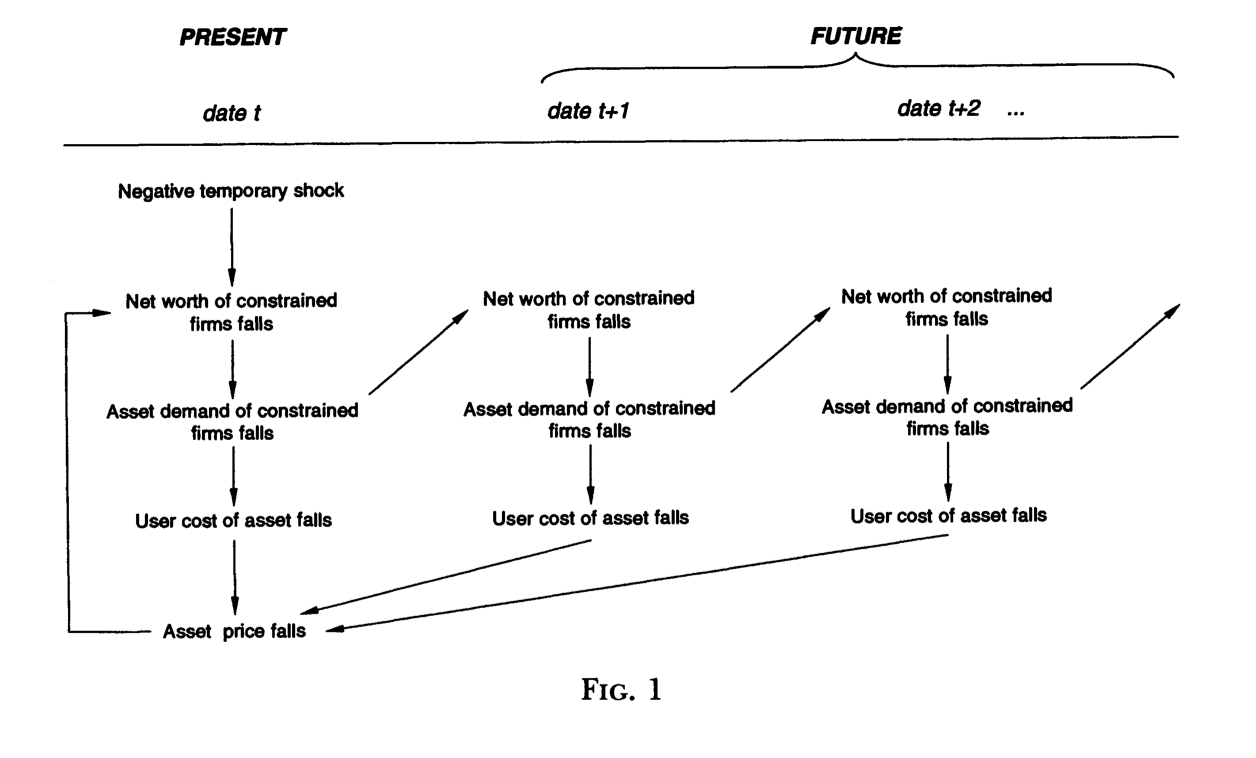
\includegraphics[width=\textwidth]{kiyotaki-moore-97.png}

\noindent
\textbf{Skills:}
\begin{itemize}
	\item How they deal with specific-targeted loan (i.e. the loan can only be used to purchase land)
\end{itemize}


% section collateral_constraints (end)


\section{Gorton and Ordonez, 14 AER} % (fold)
\label{sec:gorton_and_ordonez_14}

\textbf{\bibentry{10.1257/aer.104.2.343}}\\


\textbf{Motivation}: How a small shock can sometimes have a very huge, sudden effect, while at other times the effect of the same size shock is small or nonexistent. Leverage per se is not enough to explain this. This paper explains how credit booms arise, leading to financial fragility where a small shock can lead to huge consequences. Thus, "tail risk" is endogenous. The same reason causes boom and huge recession, and the degree of recession is positively correlated with the boom lasting time.

\textbf{Mechanism}: 

\begin{enumerate}
	\item Firm needs land as collateral to borrow money from households. Land is either good or bad. Neither firm nor household know the quality of land, and checking fee is $\gamma>0$. It can be shown that, when the probability of a land to be good is too high or too low, it will be optimal (for both firm and household) to not check the quality.
	\item Then suppose there are idiosyncratic shocks to land. For each land in each period, there is $\lambda$ prob to be unchanged, and $1-\lambda$ to be changed. In case of changing, $\hat p$ prob becoming good and $1-\hat p$ becoming bad, independent of initial type. So we can take it as a $\hat p$ type, it will become either 0 or 1 after checking. If $\hat p$ lies in some range that no checking is appropriate, then uncertainty in the economy will accumulate. Notice such accumulation will lead to a boom.
	\item Now think of an aggregate shock. All good type and $\hat p$ type have weaker beliefs after such shock, changing to $\eta$ and $\eta \hat p$ respectively. Notice that $\eta$ and $\eta \hat p$ may have very different effect. It may be optimal to not check with $\eta$ but optimal to check with $\eta \hat p$. Thus if an economy has accumulated a large portion of $\hat p$, i.e. a long boom, then many of them will choose to check, inducing a huge crisis.
	\item Notice that it is not because of any \textit{intrisinc} change in economy. The $\hat p$ will change the real portion of good land in the economy only once. What really matters is that once the bad one becomes $\hat p$, then even it switches back to bad in following periods, it will still be taken as $\hat p$. That means, the $\hat p$ type will accumulate in the economy.
\end{enumerate}

\textcolor{red}{Why this paper is important}:
\begin{itemize}
	\item Provide a way to endogenize information in general equilibrium model.
\end{itemize}


% section gorton_and_ordonez (end)

\section{Williamson, 87 QJE} % (fold)
\label{sec:williamson_87_qje}

\textbf{\bibentry{10.2307/1884684}}\\

\cite{10.2307/1884684} mainly wants to explain two things:
\begin{itemize}
	\item Why is debt contract so popular?
	\begin{itemize}
		\item By MM Theorem, we know that in a frictionless world, debt contract is equivalent to equity contract. But we notice that most fund is raised through debt.
		\item Explain by moral hazard. Borrower has private information on outcome. And lender has to pay for checking.
	\end{itemize}
	\item Why there is credit rationing?
	\begin{itemize}
		\item If the borrowing demand exceeds lending supply, why doesn't the interest rate increase to clear the market?
		\item Because checking is costly, so incentive compatibleness requires interest rate not being too high.
		They prove that the optimal interest rate is hump shape.
	\end{itemize}
\end{itemize}

An IC contract $\{S,K(w),R(w)\}$ contains three parts. $S$ is the checking area. $K(w)$ is the transfer to lender when not checking. $R(w)$ is the transfer to lender when checking. Since the contract is IC, so the reported $\hat w$ is just actual realized $w$.

There are three steps to prove the optimal contract is debt contract in this asymmetric information case.
\begin{enumerate}
	\item Prove $K(w)$ equals a constant x. [easy]
	\item Prove the IR constraint of lender will be tight. [easy]
	\item Prove $R(w)=w$, i.e. lender will take away everything in checking case. [difficult] 
\end{enumerate}

In the third step, the idea is easy. Because if lender takes away everything in checking case, then the checking area can be smaller, thus can save checking cost. The difficulty is: when we lower x (to make checking area A smaller), the non-checking area B becomes larger. The changes are in two different directions and problem becomes subtle. \textcolor{red}{In discussion we use the total differentiation approach to solve this. Important}.\\

\noindent
\textbf{Techniques:}

\textbf{how to prove optimal contract format:}

See above.\\

\textbf{recursive structure in defining EQM:}

One difficulty in determining the optimal contract is how to characterize outside options of lender. In equilibrium, When a lender decides whether to accept a contract from a specific borrower (entrepreneur), his outside option should be market interest rate $r$. Because entrepreneur can't identify lender, and all entrepreneur are homogeneous ex ante, so if the expected return from a specific contract should be larger than mkt interest rate $r$. Thus the IR of lender is:

\[\int_A R(w)d(F(w))+\int_B xd(F(w))-\gamma Pr(A) \geq r\]

$r$ has to be pinned down in the eqm. Because all agents have rational expectation, thus the market clearing $r$ will be the same as their expectation.

The equilibrium is defined as:
\begin{itemize}
	\item 
\end{itemize}


% section williamson_87_qje (end)


\section{Chari et.al, 14 AER} % (fold)
\label{sec:chari_et_al_14_aer}

\textbf{\bibentry{Chari_etal2014:aer}}

\vspace{3mm}
\noindent
\textbf{Empirical Facts:}
\begin{itemize}
 	\item simultaneous fluctuation between secondary loan market and underlying land market
 	\item persistence of collapse in secondary loan market trade volume
 \end{itemize}

 \noindent
 \textbf{Main Mechanism:}
 \begin{itemize}
 	\item adverse selection AND reputation
 	\item key assumptions:
 	\begin{itemize}
 		\item agent (bank) types persist over time
 		\item players are non-annonymous (possible to build reputation)
 	\end{itemize}
 	\item adverse selection: can account for trade volume fluctuations correlated with underlying collateral value
 	\item reputation:
 	\begin{itemize}
 		\item wihout reputation concern, adverse selection will be solved quickly. Because the first stage features a separating equilibrium
 		\item with high enough reputation concern (patient enough), first stage cannot be fully separate, so adverse selection problem persists
 	\end{itemize}
 \end{itemize}



% section chari_et_al_14_aer (end)





\section{Euro Crisis} % (fold)
\label{sec:euro_crisis}

This section is based on a course material of Wang Jue. Basically it discusses the theoretical concerns of Optimal Currency Area (OCA), why Europe adopts it, its success and its failure, and the recent Euro crisis.\\

\textbf{\bibentry{Krugman:2012eu}}

\cite{Krugman:2012eu} discusses the crisis of Euro area. Based on OCA theory by Mundell, there are two big things to look at: \textbf{labour mobility} and \textbf{fiscal integration}. Because areas are likely to suffer local idiosyncratic shocks. 
\begin{itemize}
	\item Without labour mobility, a state has to make wage fall to restore the full employment, this will be much easier with its own to devalue. But if labour mobility is high, then workers can just move to other states.
	\item Fiscal integration will also help. First because federal transfer is like a insurance, also because the borrowing cost for federal gevernment is much lower.
\end{itemize}
The Euro crisis faces challenges in both parts.
\begin{itemize}
	\item The labor mobility is not high enough.
	\item No fiscal integration. And the asymmetric shock is so severe, making fiscal burden so large that calls government solvency into question. (e.g. in Spain and Greek)
	\item The bank issue. There is no `last resort', so the fear of sovereign default undermineds confidence in private banks which hold these bonds. This is called \textit{doom loops}.
	\begin{itemize}
		\item Compare between euro area countries and pegged-to-euro countries. Austria and Finland uses euro, but Finland just pegged to euro. This flexibility makes interest rate much lower during the crisis.
	\end{itemize}
\end{itemize}

\vspace{2mm}
\textbf{\bibentry{baldwin2015eurozone}}


\section{Seminar Notes} % (fold)
\label{sec:seminar_notes}

\noindent
\textbf{Cryptocurrency}

\begin{itemize}
	\item By Jesús Fernández-Villaverde and Daniel	Sanches 2017
		.Use Lagos and Wright (2005) framework.
	\begin{itemize}
		\item \url{http://economics.sas.upenn.edu/~jesusfv/Cryptocurrencies.pdf}
		\item Not positive on private currencies. First, competitive private money will not provide price stability, either with a profit-maximizing entrpreneurs or through automaton.
		\item Even with price stability, value of private moneis may go zero in infinite equilibriums.
		\item Purely private money system does not provide social optimal quantity of money.
	\end{itemize}
\end{itemize}

% section seminar_notes (end)



% section euro_crisis (end)


\chapter{Methodology} % (fold)
\label{cha:methodology}

\noindent
\textbf{Reductionism, and Micro Fundations of Economics:}

Economists are fascinated in forming `micro fundations' for almost all models. But do we really need this, does this effort pay? 

As pointed in famous paper \cite{anderson1972:science}: `\textit{The ability to reduce everything to simple fundamental laws doesn't imply the ability to start from those laws and reconstruct the universe... At each level of complexity entirely new properties appear... There is no useful parallel to be drawn between the way in which complexity appears in simplest cases of many modies and chemistry and culture ones.}'
The aggregated economy is so complecated that may not be reduced to individual decision problems.
\footnote{Zhao Dingxing has an article discussing this problem.

See \url{https://www.evernote.com/l/ATUOIdQb8hBM5r3QQv8cTK52Amq4-qlwb0E}}

Another problem worth thinking is the relationship between Sonnethein-Debreu theorem and macro economics models.

\vspace{3mm}
\hrule
\vspace{3mm}

\vspace{3mm}
\noindent
\textbf{Meaning of Decision Theory:}

(This part is heavily influenced by Henrique's class.)

Why we need to do decision theory?
Take an \textit{inverse engineering} perspective.
Suppose we have a model, which uses utility function to describe people's decison choices. 
That is, $u:X \rightarrow \R$.
And we define $C(B)=\argmin_{x\in B} u(x)=
\{x\in B | u(x)\geq u(y),\forall y\in B\}$.
We can map such functions to a \textit{equivalent class}, and can further map it to a \textit{preference relation} (a subset of relations).

The problem is such mapping is not surjective.
Every utility function has a corresponding equivalence and a prefence relation,
but there is some preference relation that cannot be represented by a utility function.
Thus we need to put some restrictions over preference relation.

The first relation is that the cardinality of indifference curves cannot be larger than $\R$.
This is easy to understand.

But this restriction is not enough.
Think of lexicographic preference,
every point in the two-dimension space is a indifference class.
The cardinality of which is $R^2$, equivalent to cardinality of $\R$.
But we know that such preference do not have a corresponding utility function.
We can further restrict preference to \textit{order separable} relations,
then by Debreu Thm, we can show the \textit{iff} between utility and preference relations.

\begin{defn}[Order Separable]
A preference relation defined over $X$ is order separable if $\exists Y \subseteq X$ countable s.t. $\forall x_1,x_3 \subseteq X$,
we have $x_1 \succ x_2 \Rightarrow \exists y \in Y$
 s.t. $x_1 \succ y \succ x_2$.
\end{defn}

Important here is thaat by assuming the range of utility function is $\R$ (such a weak condition),
we actually put some restrictions over preference.

\vspace{3mm}
\hrule
\vspace{3mm}

\vspace{2mm}
\noindent
\textbf{Calibration:}

\noindent
Why use calibration instead of estimation?
\begin{itemize}
	\item Because we live in a `tenth-best' world, and our model only catches a small part of the world.
	Use calibration we can fit the moments that our model fail to catch,
	in this sense to be more accurate.
\end{itemize}

May use calibration parameters as an intuitive check of whether the code we wrote is correct.


\myline

\noindent
\textbf{Research Reproducibility}

\cite{Maniadis:2017gq} claims two aspects of reproducibility problem.
First, it can be seen as an `evidence game', 
where researchers have some private information
and evaluators have to design a incentive compatible mechanism for publishing and granting.
Second, empirical methods from meta-research may help. 
(I don't understand the second part.)

\cite{Maniadis:2017hi} in the same issue provides more detailed guide on what will affect the credibility of scientific research.
It raises a concept post-study probability,
\[PSP=\frac{(1-\beta)\pi}{(1-\beta)\pi+ \alpha(1-\pi)}\]
where $\alpha$ is significance level, $1-\beta$ is power,
and $\pi$ is the probability that a research question is actually true. $\pi$ can be think of as \textit{prior} given by theory.
This is the fraction of `truly true and reported true' divided by `all reported true'.
Easy to see, when $\pi$ is low, 
the PSP can be very low even with low $\alpha$.
This indicates that with those fields where theory can provide little guide,
we have to be very skeptical to the `rejection' outcomes.
They are very likely to be `false positive'. 




% chapter methodology (end)









% chapter macro (end)
\part{Mathematics}

\chapter{General (mathematical) Skills} % (fold)
\label{cha:general_mathematical_skills}

\section{Log-Linearization}

\noindent
\textbf{Motivation}

Why we need log linearizations?
Because for most nonlinear discrete dynamic programming problems,
we fail to find a closed solution.
Thus we have to use numerical method or to find a approximation.
By using log-linearization,
we transform the nonlinear problem to a linear problem (around the steady state),
and we know how to solve the linear diffrence equations.

Another advantege of log-linearization is,
the new variables are in forms of $\frac{x-x^*}{x^*}$,
which is interpretable.\\


% subsection: how to do log-linearization
\subsection{How to do Log-Linearization}

Log linearization is a common method to approximate non-linear function using Taylor expansion.

When we do linearization in macroeconomics, one key is to find \emph{\textbf{steady state}} of the model.
Then we do linearization aroud the steady state.

The basic idea is, for functions like:
\[f(x)=\frac{g(x)}{h(x)}\]

take log in both sides:
\[ln(f(x))=ln(g(x))-ln(h(x))\]

By Taylor expansion, for a smooth function f(x) we have:
\[f(x)=f(x^*)+\frac{f'(x^*)}{1!}(x-x^*)+o(1)\]

Thus 
\[lnf(x) \approx lnf(x^*)+\frac{f'(x^*)}{f(x^*)}(x-x^*)\]

The above follows from the fact that $\frac{dln(f(x))}{dx}=\frac{f'(x)}{f(x)}$. Thus,
\[lnf(x)-lnf(x^*)=\frac{f'(x^*)}{f(x^*)} \cdot x^* \cdot \frac{x-x^*}{x^*}\]

And the equation becomes:
\[lnf(x^*)+\frac{f'(x^*)}{f(x^*)} \cdot x^* \cdot \frac{x-x^*}{x^*}=lng(x^*)-lnh(x^*)
\frac{g'(x^*)}{g(x^*)} \cdot x^* \cdot \frac{x-x^*}{x^*}-
\frac{h'(x^*)}{h(x^*)} \cdot x^* \cdot \frac{x-x^*}{x^*}\]

\[\frac{f'(x^*)}{f(x^*)} \cdot x^* \cdot \frac{x-x^*}{x^*}=
\frac{g'(x^*)}{g(x^*)} \cdot x^* \cdot \frac{x-x^*}{x^*}-
\frac{h'(x^*)}{h(x^*)} \cdot x^* \cdot \frac{x-x^*}{x^*}\]

Dedine $\hat x=\frac{x-x^*}{x^*}$, and we are done.
\[\frac{f'(x^*)}{f(x^*)} x^* \cdot \hat x=
\frac{g'(x^*)}{g(x^*)} x^* \cdot \hat x-
\frac{h'(x^*)}{h(x^*)} x^* \cdot \hat x\]

Notice, when we use $\hat x$ in place of $x-x^*$in the approximation,
don't forget to times $x^*$ !!\\

% How to do log-linearization when there is Expectation

\subsection{log-linearization when there is expectation (An Example)}

It may be annoying to do log-linearization when there is expectation,
because in general,
log and expectation cannot switch.
But if we don't switch, we cannot do the log-linearization as previous.
For example, see Adda\&Cooper(2003) CH5, page 115.

Suppose we have the following Euler equation:

\[u'(c)=\beta E_{A'|A}u'(c)[Af'(k')+(1-\delta)]\]

where $c=Af(k)+(1-\delta)k-k'$.

These two expressions, along with the evolution of A,
defines a system of equations.

In this system, actually we do not have to take log,
but directly do Taylor expansion at $c^*$, $x^*$ and $k^*$.
We get:

\begin{multline}
u'(c^*)+u''(c^*)c^*\hat c_t=
\beta E_{A'|A}[u'(c^*)(\bar Af'(k^*)+(1-\delta))
+(\bar Af'(k^*)+(1-\delta))u''(c^*)c^*\hat c_{t+1}\\
+u'(c^*)f'(k^*)\bar A\hat A_{t+1}+
u'(c^*)\bar Af''(k^*)k^* \hat k_{t+1}]
\end{multline}


The first term in LHS and the first term in RHS cancel each other.
And we divide both sides by $u'(c^*)$, and we will get:

\begin{equation}\label{eq1}
\frac{u''(c^*)c^*}{u'(c^*)}\hat c_t
=\beta E_{A|A'}[\frac{u''(c^*)c^*}{u'(c^*)}\hat c_{t+1} \frac{1}{\beta}
+f'(k^*)\bar A \hat A{t+1}
+f''(k^*)k^*\hat k_{t+1}]
\end{equation}

Notice, we derive this based on the fact $\frac{1}{\beta}=\bar A f'(k^*)+(1-\delta)$.
Because by FOC
\[u'(c)=\beta E_{A'|A}V'(k')\]

To derive $V'(k')$, we first derive $V'(k)$,
by Envelop THM we get:
\[V'(k)=u'(c)[Af'(k)+(1-\delta)]\]

Substitute this into FOC we get:
\[u'(c)=\beta E_{A|A'}[u'(c')(A'f'(k')+(1-\delta))]\]

In this approach we fix A at the mean $\bar A$,
and thus the steady state satisfy:
\[1=\beta [\bar Af'(k^*)+(1-\delta)]\]

Here, the introduce of $\bar A$ is to describe the steady state in existence of shock.
We can see $\bar A$ as the "long term" growth of the economy,
and the we investigate what's the optimal steady $k^*$ under this long-term growth rate.

\textcolor{red}
{But I still don't know why we can cancel the expectation in the RHS.}

The equation \ref{eq1} is the linear function we want.\\

\noindent
\emph{Some Comments on the above method:}

Although it seems that the above method uses no log-linearization,
actually it does!

(to be added later)

% section log-linearization (end)


\section{Supermodularity} % (fold)
\label{sec:supermodularity}

\noindent
Reference: 
\begin{itemize}
	\item \href{run:resources/sobel_supermodularity.pdf}{Sobel's Notes:} \url{http://econweb.ucsd.edu/~jsobel/205f10/notes12.pdf}
	\item \href{run:resources/monotone_comparative_statics.pdf}{A more detailed note:} \url{https://pages.wustl.edu/files/pages/imce/nachbar/monotonecomparativestatics.pdf}
	\item \bibentry{topkis1998:supermodularity}
\end{itemize}





% section supermodularity (end)



% chapter general_mathematical_skills (end)


\chapter{Probability} % (fold)
\label{cha:probability}



\section{Bayesian Statistics} % (fold)
\label{sec:bayesian_statistics}

\subsection{Bayesian Updating} % (fold)
\label{sub:bayesian_updating}

\begin{thm}[Bayesian Update in Odds]
For hypothesis $H$, data $d$ and prior odds $O(H)$. We have posterior odds 
$O(H|d) = O(H)\cdot\frac{Pr(d|H)}{Pr(d|H^c)}$,
where the second term is called \textit{Bayes Factor}.
\end{thm}

\begin{myproof}
\begin{align*}
	O(H|d)&=\frac{Pr(H|d)}{Pr(H^c|d)} \\
	&=\frac{Pr(d|H)Pr(H)}{Pr(d|H^c)Pr(H^c)}\\
	&=\frac{Pr(d|H)}{Pr(d|H^c)}\cdot O(H)
\end{align*}
\end{myproof}



% subsection bayesian_updating (end)


% section bayesian_statistics (end)


% chapter probability (end)


\chapter{Numerical Methods} % (fold)
\label{cha:numerical_methods}


\noindent
\textbf{Computation laguage:}
\begin{itemize}
	\item \url{http://economics.sas.upenn.edu/~jesusfv/comparison_languages.pdf}
	\begin{itemize}
		\item discusses efficiency of different languages
		\item hybrid language can significantly increase efficiency
	\end{itemize}
\end{itemize}

\noindent
\textbf{Matlab Speed Up:}
\begin{itemize}
	\item Microeconometrics and Matlab: an Introduction, Ch-10
	\item vectorize and preallocate values
		\begin{itemize}
		 	\item Cooper's growth model uses clever vectorizing, avoid one loop
		 \end{itemize} 
	\item profiling code: profile on, main, profile off
	\item parallel computing
\end{itemize}

\section{Numerical Maximization} % (fold)
\label{sec:numerical_maximization}

\noindent
\textbf{Newton-Raphson Method:}

Idea: use quadratic function to approaximating real function at current guess,
then find the maximization point of this quadratic function as next guess.
\[\beta_{t+1}=\beta_t + \lambda(-H^{-1}_t)g_t\]
where $H_t$ is the Hessian of the function to be evaluated at $\beta_t$, 
and $g_t$ is the Jacobian at $\beta_t$,
$\lambda$ is the step size, generally may take 1.

\vspace{3mm}
\noindent
\textbf{BHHH Method:}

Idea: almost the same as Newton-Raphson, but use the outer product to approximate Hessian.
\[\beta_{t+1}=\beta_t + \lambda(-B^{-1}_t)g_t\]
where $B_t = \frac{1}{N}\sum_{n=1}^N{s_n(\beta_t)s_n(\beta_t)'}$
and $s_n(\beta_t)= \partial P_n(\beta)/\partial \beta$ evaluated at $\beta_t$,
and $g_t=\frac{1}{N}\sum_{n=1}^N{s_n(\beta_t)}$.

Key is, when evaluated at maximum value, $s_n$ should be zero. Thus $B_t$ evaluated at maximum is the variance of $s_n$ in the sample, which is just the Hessian of the sample likelihood function.
This is just \textit{information equality}.

\begin{itemize}
	\item [\textbf{pros:}] BHHH is generally faster than Newton-Raphson near the maximum.
	Because $s_n$ have to be calculated anyway, 
	but in NR procedure we have to calculate the second derivatives as well.
	\textcolor{blue}{But seems this is not the case, in experiments BHHH always slower than Newton-Raphson.}
	\item [\textbf{cons:}] BHHH is generally slower when $\beta_t$ is far from true value. 
	Because at these points $B_t$ is not a good approximate of $H_t$.
\end{itemize}

% section numerical_maximization (end)


\begin{itemize}
	\item Root Solving
	\item Integration
	\begin{itemize}
		\item Gaussian quadrature
		\item Sparse grid
		\item Monte Carlo integration
		\begin{itemize}
			\item antithetic accelerating
			\item importantce sampling
		\end{itemize}
		\item Quasi Monte Carlo
	\end{itemize}
\end{itemize}


% chapter numerical_methods (end)


\bookmarksetup{startatroot}% this is it
\addtocontents{toc}{\bigskip}% perhaps as well


\chapter{Miscellany} % (fold)
\label{cha:miscellany}

\noindent
\textbf{Presentation:}
\begin{itemize}
	\item Always motivate very clearly, both from economics facts and from literature.
	\begin{itemize}
		\item In macro, a graph generally helps
	\end{itemize}
	\item If possible, always use a simple model at the beginning
	\begin{itemize}
		\item To pin down the concepts/definitions
		\item To show the mechanism intuitively
	\end{itemize}
	\item Understand the result both mathematically and intuitively
	\item When writing, write horizontally!
\end{itemize}


% part miscellany_ (end)


\renewcommand\refname{Reference}
\bibliographystyle{chicago}
\bibliography{paper_notes}


\end{document}
